\documentclass[tikz,border=10pt]{standalone}
\usepackage{tikz}
\usetikzlibrary{patterns, arrows.meta, positioning, calc}

\begin{document}
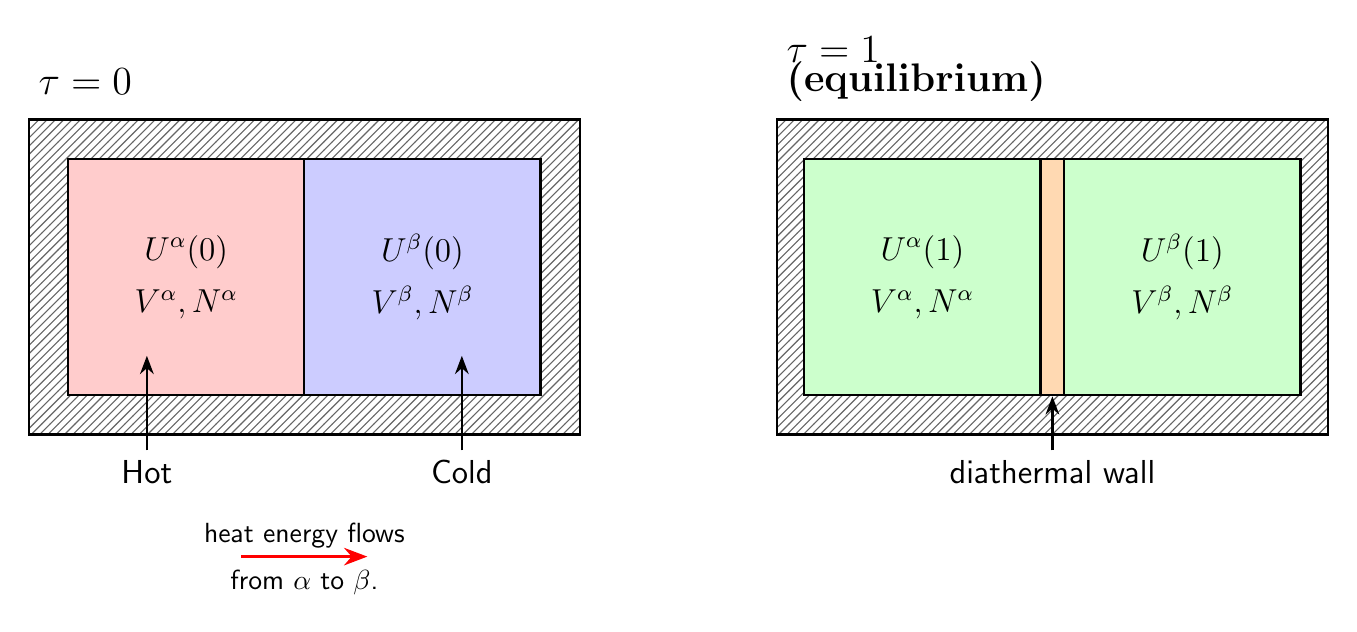
\begin{tikzpicture}
    % --- Style Definitions ---
    \tikzset{
        wall style/.style={
            draw=black, 
            thick, 
            pattern=north east lines, 
            pattern color=black!60
        },
        chamber style/.style={
            draw=black, 
            thick,
            minimum width=3cm,
            minimum height=3cm,
            outer sep=0pt
        },
        hot fill/.style={fill=red!20},
        cold fill/.style={fill=blue!20},
        equil fill/.style={fill=green!20},
        diathermal style/.style={
            fill=orange!30,
            draw=black,
            thick
        },
        title text/.style={font=\Large\bfseries},
        var text/.style={font=\large, align=center},
        label text/.style={font=\sffamily\large},
        annotation arrow/.style={
            ->, 
            >=Stealth, 
            thick, 
            black
        }
    }

    % ==========================================
    % LEFT DIAGRAM: Tau = 0
    % ==========================================
    \begin{scope}[local bounding box=leftSystem]
        
        % Title
        \node[title text, anchor=south west] at (-3.5, 2.2) {$\tau = 0$};

        % 1. Outer Wall
        \node[
            wall style, 
            minimum width=7cm, 
            minimum height=4cm
        ] (outer_left) at (0,0) {};

        % 2. Inner Chambers
        \node[chamber style, hot fill, anchor=east] (left_box_0) at (0,0) {};
        \node[chamber style, cold fill, anchor=west] (right_box_0) at (0,0) {};

        % 3. Variables
        \node[var text] at (left_box_0.center) {$U^\alpha(0)$ \\[5pt] $V^\alpha, N^\alpha$};
        \node[var text] at (right_box_0.center) {$U^\beta(0)$ \\[5pt] $V^\beta, N^\beta$};

        % 4. Standard Labels
        \node[label text, anchor=north] (lbl_hot) at (-2, -2.2) {Hot};
        \draw[annotation arrow] (lbl_hot.north) to[out=90, in=270] ($(left_box_0.south)+(-0.5,0.5)$);

        \node[label text, anchor=north] (lbl_cold) at (2, -2.2) {Cold};
        \draw[annotation arrow] (lbl_cold.north) to[out=90, in=270] ($(right_box_0.south)+(0.5,0.5)$);

        % 5. Heat Flow Annotation (FIXED)
        % Broken into separate nodes to prevent overlap
        \node[font=\sffamily, anchor=north] (text_flow_1) at (0, -3.0) {heat energy flows};
        
        % Arrow drawn explicitly between the lines
        \draw[->, >=Stealth, very thick, red] (-0.8, -3.55) -- (0.8, -3.55);
        
        \node[font=\sffamily, anchor=north] (text_flow_2) at (0, -3.6) {from $\alpha$ to $\beta$.};

    \end{scope}

    % ==========================================
    % RIGHT DIAGRAM: Tau = 1
    % ==========================================
    \begin{scope}[xshift=9.5cm, local bounding box=rightSystem]
        
        % Title (FIXED placement)
        % Wall top is at y=2.0. We place text nicely above it.
        \node[title text, anchor=south west] at (-3.5, 2.6) {$\tau = 1$};
        \node[title text, anchor=south west] at (-3.5, 2.1) {(equilibrium)};

        % 1. Outer Wall
        \node[
            wall style, 
            minimum width=7cm, 
            minimum height=4cm
        ] (outer_right) at (0,0) {};

        % 2. Inner Chambers
        \node[chamber style, equil fill, anchor=east] (left_box_1) at (-0.15,0) {}; 
        \node[chamber style, equil fill, anchor=west] (right_box_1) at (0.15,0) {}; 

        % 3. Diathermal Wall
        \node[
            diathermal style,
            minimum width=0.3cm,
            minimum height=3cm
        ] (dia_wall) at (0,0) {};

        % 4. Variables
        \node[var text] at (left_box_1.center) {$U^\alpha(1)$ \\[5pt] $V^\alpha, N^\alpha$};
        \node[var text] at (right_box_1.center) {$U^\beta(1)$ \\[5pt] $V^\beta, N^\beta$};

        % 5. Annotations
        \node[label text, anchor=north] (lbl_dia) at (0, -2.2) {diathermal wall};
        \draw[annotation arrow] (lbl_dia.north) to[out=90, in=270] (dia_wall.south);

    \end{scope}

\end{tikzpicture}
\end{document}